
%TODO må skrives: sett av 2 dager


%todo todo todo todo todo todo todo todo todo todo todo todo todo todo todo todo todo todo todo todo todo todo todo todo todo todo todo todo todo todo todo todo todo 
%
% 	ENDRE TITTEL til "comparison and discussion".      "comparison and discussion"       "comparison and discussion"       "comparison and discussion"       "comparison and discussion"       "comparison and discussion" 
% 		-> og endre tittel på neste kapittel til "Conclution"..
% 	Når kode/design skal sammenlignes: Gå gjennom, or fiks opp appendixDifferentDoTaskFunctions.tex 	Analysen skal være her, men de relevante doTask() funksjoner skal ligge der. No ligger alle der, og på norsk..
%
%todo todo todo todo todo todo todo todo todo todo todo todo todo todo todo todo todo todo todo todo todo todo todo todo todo todo todo todo todo todo todo todo todo 




% Sammenligning:
% Oppgave 3) Compare the new concept with competing methods. The evaluation may be based on a number of specific scenarios (with respect to input data etc.).
% 	Skriv at konkurerende metoder må tolkes til SANN, siden det blir for mykje å sammenligne med fANN også. Dette er en av styrkene til KANN: Kan snakke med alle!
% 	Skriv at for å kunne sammenligne med SANN, så har eg implementert begge. Dette gjør at eg kan meir grundig sammenligne implementering av de to. 
% 		Eg blir også bedre kjendt med implementasjonen så lettere å seinere gjennomføre en vilkensomhelst test (ikkje med rammer som er satt av implementasjonen).
%
% 	- Sammenligning om implementasjon OG kjøring om: Bra/dårlig ved:
% 		- kjøring av de to
% 		- implementasjon av de to
% 		- sensor(best for KANN)
% 		- Effektivitet (teoretisk sammenligning)
% 			- sammenligning av kva som krever ressurser:
% 				SANN: Generell input, lekkasje kvar iter, 
% 				KANN: endring av kappa er det tunge ( lekkasje er med i ligninga ) : bare når nødvendig.
% 						- hente ut verdien bare når den trengs. Koster bare når det er behov (ingen uptime keep).
% 						-osv. Dette er gøy å tenke på, men no: tilbake til arbeidet..
% 		- Sammenligning KANN vs SANN : heilt anna fokus for når nodene fyrer. For SANN har vi en reaktiv variant, der vi reagerer når noden går over terskel, for KANN har vi en proaktiv variant, som 
% 			beregner når den vil fyre, og bare ligger å venter på dette. 		--Her må man også diskutere/sjå på om dette er bedre for effektivitet. Ikkje heilt sikkert..
%
%
% 		- kjøretid (effektivitet for ulike 'scenarios') - DISKURS
% 		- over nettverk : best for KANN. 				- DISKURS
%


% - Sammenligning: Snakk om forskjellen i når aktivitetsVariabel propagates. Dette kan sikkert diskuteres mykje..

% TODO TODO T0D0:
% Verifiser all koden som står i teksten.



%Intro til kapittelet:
%	Intro: oppsummere kva som er gjort i dette prosjektet:
%		- Modellere neuronet.
%		- Utvikle KANN (som resultat av ligninene fra over)
%		- Utvikle SANN. Laga selv for best å kunne sammenligne forskjellene.
%		For begge ANN:  Sterk inspirert av biologien.
%			-> i tillegg til fordelane som er nevnt tidligare: gir eit felles design for implementasjonane av de to modellane => Meir sammenlignbar.
In this project two artificial neural networks have been designed and implemented. 
For the implementation it has been focused on comparability, both in respect to the design of the simulation and the behavior of the indivitual node.
The systems will be more comparable if both systems have the same blueprint. 
This is one of the reasons why the implementations are so inspired by biology.
An other cause for the strong resemblance with the biological neuron is the recognised connection between each generation of ANN; As ANN models evolve, each generation become closer to the biological version. %skriv om xxx.
This observation is a strong motivation of make the impementation close to the biological neuron, as long as it does not affect the effectivity of the simulator. %bruk fleire setninger?
%The comparability in design and implementation it the cause of an, in some cases, overly complicated object model.

For comparing the behavior of the indivitual nodes of the two nodels, some effort was put into a capabel logging system. 
Different elements of the node with interresting variables of effects were logged by this system. This includes the \emph{K\_synapse}, the \emph{K\_auron} and the \emph{s\_auron}.
The synapse was logged mainly for design purposes. The two auron elements were logged for design purposes and for the ``depolarization'' value comparison.
Both auron models is able to write the ``depolarization'' to a log file. The $\kappa$N is also able to log it's activity level, through $\kappa$.

The activity level of a spiking neuron us not formalized; Neuroscientist often use variables such as the firing frequency to measure the activity of a neuron.
For this reason, no method has been implemented for logging the activity level of the SANN nodes.
The activity of the single node is a phenomenon that first becomes important when we analyze larger neural networks.
For the comparison of the single node, the value of the node is the best comparison variable. 
%This containt more information, and if analyzed also contains information of the firing frequency and the synaptic input of the node could be found.
In this report it is most interresting with the transient depolarization curve of the nodes.




\section{Comparison of Design and Implementation for the Two Models}

	% Begynn med å oppsummere korleis objektmodellen er lagt opp.
	% Gå gjennom de ulike elemena? Auron -> dendrite -> osv. ? 	 (HUSK Dette er bare innledning: skal være en ekte delmengde av det som kommer, (delmengde som ikkje er det samme), DERMED: IKKJE SKRIV ALT ("hold spenninga oppe").
	% (Skriv om ulikhetane i variabler. Bare såvidt nevn ulikhetane i funksjoner..)
	% 	[Slik:] For the auron, not much could be put into the common interface class of i_auron ...
	% 			For the axon, on the other hand ...
	% ANDRE forskjeller: (designforskjeller)
	% Design av de to implementasjonane er gjordt som en direkte simulering av neuronet (spiking neurons), med dendrite, axon, osv. 
	% 	Dette førte til at eg begynte å impelmentere de to som like, bare med peiker-funksjoner for de funksjonane som trenkte å være ulike.
	% 	Eg oppdaga raskt at dette ikkje ville fungere, siden nesten alt er ulikt fra SANN til KANN.
	% 	Endte opp med å ha en interface class for kvart element (i_[element]) som arva til de to modellenes design av elementet (s_elemen og K_element).
	% 		Dette førte til at forskjellane i design ble veldig tydlige. Fellestrekka for de to modellane ble også veldig tydlige.
	% nevne det som står kommentert ut i section{Design for each node, ...} ?
	%
	% Nevn også at objektmodellen la opp designet (for begge modellimplementasjoner), og eg oppfatta først etterpå at dette kunne gjøres langt meir effektivt for KANN.
	%  

	In this project, both implementations were designed to make the differences stand out.
	The nodes were designed as the biological neuron, both to give a common design to both models and to make the design more recognizable for the reader with knowledge of neuroscience.
	All common aspects of the subelements of each node was placed in an abstract class derived to the model--specific classes.

	The abstract interface class were named \emph{i\_[element]}, and the model--specific class was named \emph{s\_[element]} for the SN and \emph{K\_[element]} for the $\kappa$N.
	Here \emph{[element]} can be one of the four elements each node consists of; The dendrite, the auron, the axon or the synapse.

	As the design made it possible to place all similarities for the two models in the common abstract \emph{i\_element} classes, the similarities and differences between the models became prominent.
	%In this section some of the similarities between each element will be presented.
	
	In this section the results will be presented.  %TODO TODO TODO TODO TODO TODO TODO TODO TODO TODO TODO TODO  ENDRE avslutting av intro.
	This will start by presenting a comparison between the individual elements before presenting a larger view of the differences between the models. % TODO Sjekk at dette er rett. Endre setning når section er skrevet..

	\subsection{The activity level}
	
	The largest and most immediate difference between the two models is how the activity level is represented.
	The SANN model is a direct simulation of the depolarization of the neuron. 
	Synaptic input alters the value of the node, and if the value goes above the firing threshold a simulated action potential is fired.
	The value of the node is modelled as a leaky integration of the node's input, and each time iteration we have a little dissapation of the value.

	For the $\kappa$ANN model, use higher order mathemathics to calculate the firing time of the node.
	The neuron is modelled as a LIF neuron, and the leaky integration is included in the equations used by $\kappa$ANN.
	In these equations we calculate the firing time of the node, given a constant level of input until firing of the node. 
	%As the equations from sec. \sec{secMatematiskModelleringAvBioNeuron} requires a constant activity level, the concept of a time window was introduced.
	
	The activity variable of a $\kappa$N is based on the notion of the final value of the simulated depolarization value of the node.
	Given a constant level of input and a constant degree of leakage, the value of the node will converge to some value $\kappa$.
	By the use of this value, the period of the node is calculated.

	As the variable sertainly will change before the end of some period, the concept of a time window was introduced.
	The concept of the time window gave the oppurtunity to use the model in an artificial neural network, if the state of the node was calculated each time the activation level was altered for the node.
	%MEIR XXX


	\subsection{Information propagation}
	Synaptic transmission can be said to give the transmission of the activity of one node to the next.
	As the activity variable of the node differs between the two models, synaptic transmission is also different for the two models.

	In a SN, the transmission directly alters the postsynaptic value of the node.
	As for every other aspect of SANN, synaptic transmission is a direct simulation of the relevant aspects of the biological equivalent.
	An excitatory artificial synaptic thus increase the postsynaptic activation level and an inhibitory artificial synapse decrease the postsynaptic activation level.

	For the $\kappa$N, the activation level is a consequence of the level of input to the node.
	As the presynaptic node is capable of esmimating the future firing frequency of the node, synaptic transmission between two nodes is given by this frequency scaled by the synaptic weight.

	The activity variable of a $\kappa$N is a time--invariant variable, as the final value of the node does not dissapate with time;
		The final value of the node will stay the same, given a constant level of input.
	Each transmission is therefore a time invariant signal, and the postsynaptic node's activity variable can be recalculated at any time.
	The postsynaptic activity level could therefore be calculated as the sum of all synaptic input transmissions after the transmissions in one input synapse is altered.

	For the sake of efficiancy, the concept of the edge transmission as the derived is used in this implementation.
	In this case the postsynaptic activity variable could be updated by adding the edge transmission to the postsynaptic activity variable.
	The strenght of the time invariant signal became appearent when the activity variable $\kappa$ was recalculated to avoid to large global trunctation errors.


%	In this section, some of the similarities and differences between each node element is presented.
%	The activity level of the two models differs tematically.
%	For a SN, the activity level corresponds to the simulated depolarization of the node, while for the $\kappa$N the activity level 

	%Meir
	
	\subsection{Comparison of the indivitual node elements}
	%	%todo SKRIV OM! Innledning til section
	%In this section, some of the similarities and differences between each element of a node will be presented.
	%
	%The result will be presented in the order the signal propagates through a node.
	% 	%First the difference in synaptic transmission will be presented.
	%We will start out by taking a look at the differences in synaptic tranmission; 
	%	What is transmitted and how the sigal affects the postsynaptic node.
	%When synaptic transmission for the two models has been introduced, the mechanisms of the signal propagation within each node will be discussed.
	% 	%As the mechanisms of the activity of each node differ strongly, the activity variable of each node is 
	% 	%The difference in the activity level of each node differs strongly, as a resu
	%This section will be concluded by listing the similarities between the two models. 

	As the elements of each node was designed by having a common abstract class derived to the two modes, the aspect that was different between the SN and the $\kappa$N stands out clearly.
	The aspects that are similar between the models is represented in the common interface class.

	In this section, the differences in design for the indivitual elements of the two model--specific nodes are presented. %TODO Dårlig setning!
	The results are presented in the order of the signal propagation within each node.
	
	The elements are compared by the function that defines the element's behaviour in time, the \emph{timeInterface} derived virtual function \emph{doTask()}.
	As this is what defines the action of the node, the design of this implementation isolates the location of the differences between each model--specific element. %XXX BLABLA TODO Fullfør.
	%Vettafaen om eg trenger intro i subsection.. XXX 	 (?) Ta vekk:
	%First the mechanisms of signal transmission will be presented, by comparing the two synapse designs.
	%The results for the difference in dendritic integration of all input synapses transmission will then be presented.

		\subsubsection{The Mechanisms of the Synapse Element}
		We can sum up the previous discussion of synaptic transmission by saying that the activity variable of the nodes, and thus what is transmitted in a synaptic transmission is tematically different.
		In the SN the node variable is the immediate %[kor han er]  along the path toward firing.
		For the $\kappa$N the activity variable gives the activity level of the node.

		This shows in the implementation of the two models' synapse functions.
		When the \emph{s\_synapse} executes a synaptic transmission, it adds the synaptic weight to the postsynaptic node's activation variable.
		As stated in in section \ref{secSANN}, the SN is a direct simulation of the elements of the biological neuron.
		This can be seen if we compare the workings of the synaptic transmission in the \emph{s\_synapse} with the biological synapse, introduced in sec. \ref{ssecTheSynapse}.

		For the $\kappa$N, synaptic transmission is given by the presynaptic node's frequency and the synaptic weight.
		The edge transmission is further defined as the derived of the synaptic transmission in this implementation.
		When the postsynaptic node updates its activity variable, this is done by simply adding the edge transmission to its activity variable.
		% XXX SKRIV OM : We end up with the same transmission scheme, but the variables is 
		
		%TODO Skriv heilt om eller ta bort:
		%The code for the implementation of the two element's \emph{doTask()} function is included in appendix \ref{appendixDoTaskForSynapse}.
		%We can see the difference in synaptic transmission clearly from the code.

		One important difference between the models becomes obvious allready in synaptic transmission.
	%	As the synapse transmits a value that varies with the presynaptic activity level, and that the postsynaptic activity level is given by this signal, we could say that this is a 
		%One important difference in the synaptic tranmission between the two models is therefore that the synaptic transmission of the $\kappa$N 
		The size of transmission in the $\kappa$N varies with the presynaptic period, further given by its activity variable.
		As the activity variable is given by the immediate input of the node, we get that the output transmission is given by the state and the input of the node.
		We could say that the $\kappa$N is a Mealy automata of the biological neuron.
	
		%TODO Skrive at SN er en moore modell? (i forhold til siste linja over).

		%Skriv om tematisk forskjell: KN overfører variabel som eg gitt av nodens inputlevel..

		\subsubsection{The Mechanisms of the Dendrite Element}
		%Both the SN and the $\kappa$N is implemented as the derived of the postsynaptic activity variable.
		For both the SN and $\kappa$N, synaptic transmission gives the derived of the postsynaptic activity variable.
		The input to a node thus gives the same result \emph{for the activity variable} in a SN and a $\kappa$N.
		%For the activity variable, a new input therefore gives the same result for the $\kappa$N and the SN. 
		%Both \emph{newInputSignal(double)} adds the new input to the the activity variable.
		
		In SANN, the dendrite first has to see whether the postsynaptic node is in a refraction period. 
		%For the SN, the dendrite first have to chech that the node is not in a refraction period. 
		If not, the dendrite starts to execute the algorithm of the postsynaptic part of synaptic tranmission.
		Prior to adding the new signal to the postsynaptic node's value, the dendrite calculates the leakage.
		This is done by eq. \eqref{eqLeakageForSANN}. 

		As the postsynaptic node will fire an action potential as soon as the value of the node goes above threshold, 
			the \emph{newInputSignal(double)} function has to test this as a part of its algorithm. %the incmng signal transmission.

		%If not, the dendrite calculates the leakage since the last time the leakage was calculated, before it adds the new input signal.
		%as the postsynaptic node will fire an action potential if the value goes above the threshold, this is checked by the synapse in the \emph{newInputSignal()} function.

		If a delay is modelled into the simulation, the action potential is initiated after $n$ time steps, were $n$ is the predefined delay.
		This is best done by letting the dendrite insert the first element in a linket list of $n$ elements into \emph{pWorkTaskQue}.
		%If $n$ is a number larger than one, $n$ elements will have to be in series before the axon hillock, for the \emph{s\_auron}.

		For the $\kappa$N, the activity variable is time--invariant; From eq. \eqref{eqKappaSomFinalValueAvV} we get that $\kappa$ is the final value of the node, given a constant input.
		%In the LIF neuron, this final value does not change as a 
		As $\kappa$ is time--invariant, nothing has to be calculated as a result to time alone. We can therefore effectively use an event--based simulation scheme.
		%This further gives that nothing has to be calculated as a function of time alone. 

		By the scheme of edge transmission as the derived of the synaptic transmission, we can calculate the postsynaptic activity variable by simply adding the edge transmission.
		%	the edge transmission only has to be added to the postsynaptic activity variable.
		As the $\kappa$N calculates future firing time by the activity variable, we do not have to check the postsynaptic activity variable after each transmission.
		For the $\kappa$N, most of the operations of SN transmission is therefore avoided:
			%we therefore have that most of the operations for the SN dendrite input is avoided: 
		\begin{itemize}
			\item The leakage does not have to be calculated
			\item It is unnessecary to compare the activity variable to the firing threshold
			\item The simulation of intracellular transmission delay becomes obsolete. Simulation of delay can be included in the calculation of the firing time of the node.
			\item As firing is controlled by other mechanisms, no elements is inserted into \emph{pWorkTaskQue}
		\end{itemize}
		If a predefined delay of $n$ time steps is to be included in the simulation, in $\kappa$N this is done by directly adding $n$ to the estimated firing time of the node.

		If we take a look at the two \emph{newInputSignal(double)} functions, listed in appendix \ref{appendixNewInputSignalDendrite}, we can note that the $\kappa$N version is substantially smaller.
		The size can, however be decieving, so we will now discuss the two functions.
		%skriv om at calculateLeakage er stor operasjon. Med exp-funk
		The SN dendrite calls the function \emph{calculateLeakage()} and the $\kappa$N calls the \emph{changeKappa\_derivedArg()} function.
		The \emph{calculateLeakage()} function will calculate the leakage as a result of the time since the last calculation. 
		This is doen by equation \eqref{eqLeakageForSANN}.
		
		For the $\kappa$N, dendrite calls the model--specific \emph{K\_auron::changeKappa(double)} function.
		%This will be discussed in XXX SKal eg diskutere dette i auron?
\begin{lstlisting}
inline void K_auron::changeKappa_derivedArg( double dInputDerived_arg)
{
	// add arg to Kappa
	dChangeInKappa_this_iter +=  dInputDerived_arg ;

	// Insert [this] pointer to pCalculationTaskQue
	time_class::addCalculationIn_pCalculatationTaskQue( this );

	writeKappaToLog();
}
\end{lstlisting}

		As we can see, the $\kappa$N uses the concept of \emph{pCalculatationTaskQue}.
		Whenever $\kappa$ is changed, the node is scheduled for recalculation of all the values that is given by $\kappa$. %a new input changes $\kappa$, 
		Exampes of this is the corresponding frequency to the present $\kappa$ and the estimated firing time. 
		Changing $\kappa$ will also initiate a new time window.

		Due to the mechanisms of \emph{pCalculatationTaskQue}, this will only be done once for any time iteration.
		The calculations will be executed as the last action before time is iterated.

		% TODO VIKTIG Skriv at diskurs over gir at KN kalkuleres det meste bare en gang. For SANN sjekkes alt kvar gang vi har input.
		The difference in efficiancy between the two models will therefore depend on the number of inputs per time iteration.
		For the $\kappa$N we execute the heavy part of the calcutaion (at most) once every time iteration. 
		The other part of synaptic transmission is based on adding the edge inputs to the postsynaptic activity variable.

		For the SN, apart from the calculation of leakage, the same amount of work is done every time the node gets an incoming synaptic transmission.
		%Apart from the calcutaion of leakage, the same amount of work is done every synaptic transmission for the SN.
		%Elements of this work is the general amount of actions, the three if--sentences that break up pipelining in the processor (there is also one inside the inlined function \emph{calculateLeakage()}).
		%
		%As this amount is not insubstantial, the $\kappa$N could be more effective for a large part of the 
		This amount is given by two aspects, where the most important probably is the three if--sentences (two in the listed code and one in the inlined function \emph{calculateLeakage()}).
		Each if--sentences will break up the pipelining of the processor, and lead to a decrease in the efficiancy of the execution.

		\subsubsection{The Mechanisms of the Auron Element}
		The auron is the central element of each node, and contains the central mechanisms for signal propagation.
		For the SN, this includes the depolarization variable (\emph{dAktivitetsVariabel}) and the time stamp used for the calculation or leakage. %og fyrin av AP.
		For the $\kappa$N, this includes $\kappa$ (\emph{dAktivitetsVariabel}), the initial value for the depolarization and initial time iteration in the current time window and a variable containing the calculated period inverse.
		The variable that contains the present period inverse is used for calculation of edge tranmission when $\kappa$ is changed.
	
		% TODO TODO TODO TODO TODO TODO TODO TODO TODO TODO TODO TODO TODO TODO TODO TODO TODO TODO TODO TODO TODO TODO TODO TODO TODO TODO TODO TODO TODO TODO TODO TODO TODO 
		% TODO TODO TODO TODO TODO TODO TODO TODO TODO TODO TODO TODO TODO TODO TODO TODO TODO TODO TODO TODO TODO TODO TODO TODO TODO TODO TODO TODO TODO TODO TODO TODO TODO 
		% TODO TODO TODO TODO TODO TODO TODO TODO TODO TODO TODO TODO TODO TODO TODO TODO TODO TODO TODO TODO TODO TODO TODO TODO TODO TODO TODO TODO TODO TODO TODO TODO TODO 
		% TODO TODO TODO TODO TODO TODO TODO TODO TODO TODO TODO TODO TODO TODO TODO TODO TODO TODO TODO TODO TODO TODO TODO TODO TODO TODO TODO TODO TODO TODO TODO TODO TODO 
		% TODO TODO TODO TODO TODO TODO TODO TODO TODO TODO TODO TODO TODO TODO TODO TODO TODO TODO TODO TODO TODO TODO TODO TODO TODO TODO TODO TODO TODO TODO TODO TODO TODO 
		% SKRIV MEIR!

		\subsubsection{The Mechanisms of the Axon Element}
		The axon is where the difference in execution is most prominent.
		In absence of a suitable timing mechanism, the SN uses the axon as a pure time delay.
		At the time of firing for the node, the axon is inserted into \emph{pWorkTaskQue}.
		Let $n$ be the number of serially linked axon elements before some output synape.
		The synapse will now get a transmission after a delay of $n$ time iterations.
		We can therefore give the time delay before transmission at a particular synapse by the number of serially linked axon elements before it.

		For the $\kappa$N, the same result can be achieved by letting the $\kappa$N write the planned execution time to to the corresponding synapse in the $\kappa$ANN version of the network.
		The planned execution time for the synapse, $t_{e, syn}$ is given by
		\begin{equation}
			t_{e,syn} = t_f+n \qquad, \; \text{$t_f$ is the firing time of the node}
		\end{equation}
		If $t_{e, syn}$ is written to the corresponding synapse in the $\kappa$ANN, the synapse's \emph{doTask()} function is executed at the same time iteration as for the SN version of the network.
		%The same result it therefore achieved for the timing of the transmission in the $\kappa$N synapse as in the SN synapse, only with a much smaller effort for the simulator.
		The same result it therefore achieved for the time of transmission for the $\kappa$N synapse as for the SN synapse, only with a much smaller effort for the simulator.
																							% TODO Del opp setninga over, | HER, (over streken) ?

	%	For some output synapse, the pointer to the synapse is inserted into \emph{pWorkTaskQue} after a predefined delay of $n$ time iterations.
	% 	The number $n$ is a consequence of the number of serially linked axon elements.

	%	Depending on the spatiotemporal resolution, the node's output synapses will be inserted into 
	%	The next time iteration (or after a number of time iterations
	%	As the SN use the axon as a meth










%XXXXXXXXXXXXXXXXXXXXXXXXXXXXXXXXXXXXXXXXXXXXXXXXXXXXXXXXXXXXXXXXXXXXXXXXXXXXXXXXXXXXXXXXX
Skrive at design av/teorien bak  de to impelmentasjonene er så forsjellig at det er vanskelig å sammenligne de to. En enkel kjøring vil ha statisk input (ikkje-endrende input).
Mealy varianten av SANN (KANN) er spesialisert for ANN med dynamisk (endrende) input. Vil gi eit vanskeligere testoppsett for sammenligning av de to. Lett å implementere for KANN, vanskeligere å implementere for SANN.
(Da må eg ha egene sensor-neuron som er spesiallaga for å sense en slik dynamisk state).
%XXXXXXXXXXXXXXXXXXXXXXXXXXXXXXXXXXXXXXXXXXXXXXXXXXXXXXXXXXXXXXXXXXXXXXXXXXXXXXXXXXXXXXXXX






%\section{Forskjell i implementasjon}
Skrive at forskjellen mellom gamle og nye varianten av 3.gen. ANN (SANN) har mykje til felles med forskjellane mellom Moore vs. Mealy Auromata.

Den gamle varianten er for så vidt den som er mest intuitiv å implementere / designe. Denne ser på umiddelbar tilstand (depol. verdi) for nodene. Dersom denne depol. kommer over terskel vil noden gi output til alle sine utnoder.
Dette er en direkte simulering av det biologiske neuronet. Kan beskrives (direkte?) med Moore Automata.

For den foreslåtte varianten vil Mealy automata beskrive systemet bedre. Her er det 'state' for noden og i tillegg input som gir ut-oppførselen.
[skriv kva "utoppførsel" betyr. Alltid samme output (før synapsen) for den Moore-Automata varianten av SANN. For Mealy variant vil output være en flyttallsvariabel]
[skriv kvifor denne tanken kom -- at enkel kraftig prosessor vil være oppmot like effektiv med større flyttalsoperasjoner som ved enkle boolske transmissjoner (tjaneei..)
Dersom vi har mulighet er ferre større operasjoner bedre for den serielle CPU enn mange små operasjoner.]

[Skriv at implementasjonen viste seg å bli meir omfattende enn først tenkt. Skriv om pEstimatedTaskTime og anna ekstra tidsplanlegging]

% TODO TODO TODO TODO TODO TODO TODO TODO TODO TODO TODO TODO TODO TODO TODO TODO TODO TODO TODO TODO TODO TODO 
%Viktig eksempel til diskurs.
		In addition, we have the aspect of \emph{how} the activity of the node changes. 
		Let us take an example where we simulate a neuron with a constant level of synaptic input.
		For the $\kappa$N, the node will have a constant activity level, and does not have to recalculate the firing time of the node when the node fires.
		When the node fires, the node writes the current time iteration plus the previously calculated period to the member variable \emph{ulEstimatedTaskTime\_for\_object}.
		When the estimated task time is the same as \emph{time\_class::ulTime}, the node fires again and the same is repeated.
		For the SN, the number of input transmissions stays at a constant level to produce the same firing frequency for the node.
		The number of actions for the SN will therefore stay at a constant level throughtout the simulated period.
		As the $\kappa$N only has to calculate its activity level initially in the example, when its $\kappa$ is changed, we get a large difference in work load for this example. 
		
		The example is unrealistic for most circuits, but it examplifies when $\kappa$ANN will be more effective than SANN.
		Even thought the example is unrealistic, there might me situations where a $\kappa$N would be better than a SN.
% TODO TODO TODO TODO TODO TODO TODO TODO TODO TODO TODO TODO TODO TODO TODO TODO TODO TODO TODO TODO TODO TODO 




% XXX MERK har skrevet det meste før (i design). Skal isåfall bare nevnes her..
Skriv også om generellt optimalisering:
\begin{itemize}
	\item flytande tid. Ikkje alle noder trengs å sjekkes kvar iterasjon. (sjå/edit det over). (SKRIV OM implemenasjonene til Ås, og at de bruker synkron tid).
	\item samle opp beregning av $\kappa$ til slutt. $\kappa$ kan endre seg fleire ganger i løpet av en iterasjon. På grunn av dette skal alle noder som får endra aktivitetsnivå legges inn i ei liste. Denne lista gåes gjennom ved tidsiterasjon (i tid::doTask() ). Skal bare ligge eit element av eit objekt i lista, så dersom $\kappa_i$ endres fleire ganger for neuron $i$, vil det bare bli en kalkulering av depol./`interspike period' per [neuron, tidsiterasjon].
\end{itemize}

Her kan også ``Firing Cycle'' stå. Dette er estimering fordi hastighet ikkje er konstant lik gjennomsnittshastighet. Dersom FC skal brukes (som optimalisering) så kan enten gjennomsnittshastigheta over heile perioden brukes, eller så kan perioden deles opp i $n$, og gjennomsnittet i kvar bit brukes (for eksempel $n=2$: deler farta inn i to deler. Først er farta stor, så blir den mindre, fordi $(1-e^{-at}$ flater ut..)

		
	%Sammenligning av design for de to modellane. Med samme output er det mulig å simulere ANN ved bare en node. Dette kan eg godt vise i plot.


% XXX TEMATISKE FORSKJELLER -- Når har vi høg load for systemet. Når kreves mykje ressurser?
	\subsection{Høgare ordens mekanismer som resultat av det over. Forskjeller..} 
	%Det kom fram at for KANN er det mulig å gjennomføre tidsdelay som kommer av axon og dendrite med bare auron-elementet.
	%Dette gjøres med å plusse på en på estimert fyringstid.. VIKTIG poeng!
	%
	% XXX Skriv om reactive vs. proactive kalkulering av fyringstid.
	\subsection{Design for each node, when designed as a simulation of temporal aspects of the neuron}
	% XXX Dette skal bare nevnes her (eller?), men skrives så utførende som teksten under, i egen section.
	% En annen ting en oppfatta var at simulering av kvart element ikkje var nødvendig for simulering av time--delay for propagering av AP: for KANN kan dette inkorporeres i estimering av fyringstid og periode (=>syn.transmitted var.)
	% 	For KANN kan man lett effektivisere bort simulering av tidsdelay, ved å bare legge til tidsdelayet i estimat av fyretid. Dette er vanskeligare å gjøre i SANN. I KANN er denne typen effektivisering "native".
	% 	Dette gir at for simulerings-likheten som er brukt i dette systemet (en dendrite, eit axon -- alle synapser samme plass..), så er det mulig med eit--elements noder for KANN uten å miste simuleringslikhet.
	% 		I implementasjonen er K_dendrite::doTask() og K_dendrite::doCalculations() definert til å gi sterk melding og avslutte programmet. Dette for å eksemplifisere at de ikkje er i bruk, og forsikre at de ikkje blir kalla.
	% 		For K_axon så gjelder fortsatt det at eg vil ha muligheten til å auke 'spatsio-temporal' oppløsning. Dette gjøres ved å legge inn fleire element av K_axon. K_axon blir dermed som eit navier--stokes kontrollvolum for neuronet.
	% 		Dersom en pragmatisk implementasjon blir laget fra denne koden, kan dermed K_axon fjærnes, of listen med output synapser og doTransmission() kan legges over i K_auron.
	% 		I såfall får vi eit enklere oppsett of kvar node, med bare eit node element (K_auron) og eit 'edge' element (K_synapse), uten å miste kvalitet i simuleringen. 
	% 		Dette kan sees i plotta som sammenligner depol-kurve for de to ANN (sjå plott[_ref_])
	
	Konkluder med å diskutere lettheten i implementasjon(at KANN er vanskeligare å implementere, men med andre pluss..) 			ELLER:   i 'discussion and conclusion' ?

\section{The Nodes' Output}
	% XXX Dette skal hovedsaklig ligge i KANN, men siste plott skal også legges ved her (eller bare her?) \subsec.{Comparison between the transient time course of the depolarization of the K auron and s auron,Vettafaen kor det skal ligge}
	%\subsection{Comparison of the transient time course of nodes of the two models}
	\subsection{Transient Time Course of The Two Model--specific Nodes}

\section{Comparison between the transient time course of the depolarization of the K auron and s auron ,   Vettafaen kor det skal ligge}
To compare %the implementation of (?)
			the two models, the the first aspects to be compared is the depolarization  of a single node of each model.
%							we will start with comparing the depolarization of a single node from each model.
The same input to the two nodes should give the same transient time course of the nodes' depolarization.

Because of the complexity of the single node, we cannot use a network of neurons to generate an equal input to the analyzed neuron. 
At least not before we know that the two model--specific nodes give the same output. %TODO Skriv om. Litt.
%The solution for this problem was to design an underclass 
%My solution for this was 
% TODO TODO TODO TODO TODO DETTE SKAL SKRIVE I KANN.tex ATODO TODO TODO TDOO TODO TODO TODO D TODO TODO TODO TODO TODO TODO TODO TODO TODO TODO TODO TODO TODO TODO TODO TODO TODO TODO 
The solution for this problem was
									to design an own underclass K\_sensor\_auron for the $\kappa$ANN model and s\_sensor\_auron for the SANN model.
Objects of these classes continously update its activity level by the output of some ``sensor function''.
%This sensor function was designed to give an output appropriate for comparing the variants of the node.
Both sensor classes are constructed by sending a function pointer into the constructor of the object. 
The function sent in to the constructor as a function ponter could be specifically designed for the comparison in mind.

\begin{lstlisting}
K_sensor_auron::K_sensor_auron(
  std::string sNavn_Arg, double (*pFunk_arg)(void) ) 
     :  K_auron(sNavn_Arg)
{
	// Assign the sensor function:
	pSensorFunction = pFunk_arg;
	// Add to pAllSensorAurons list:
	pAllSensorAurons.push_back(this);

	...
}
\end{lstlisting}

Where the member variable \emph{double \mbox{(*pSensorFunction)(void);}} is a function pointer that is assigned the the function pointer adress that is sent in as an argument in the class constructor.
%This causes \emph{pSensorFunction} for point to the function sent in as an argument in the constructor.'
The variable pAllSensorAurons is a list containing all the valid sensor objects, used for updating the value of each sensor neuron when \emph{time\_class::doTask()} iterates time. %i time_class::doTask()

\begin{figure}[hbtp!]
	\centering
	%\begin{center}
		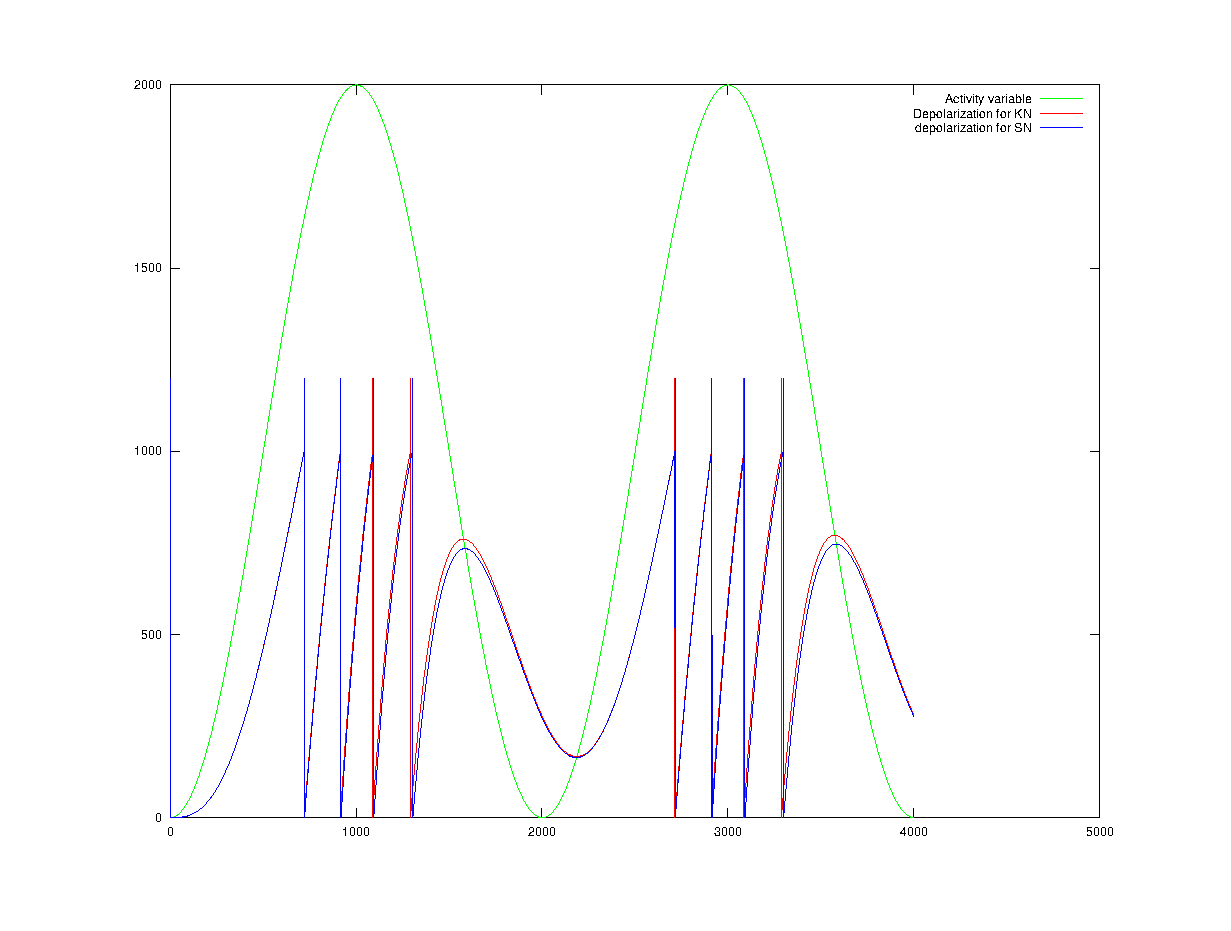
\includegraphics[width=0.95\textwidth]{eps_Comparison_between_the_two_sensors__depol.eps}
	%\end{center}
	\caption{The depolarization curve for a SANN node and a $\kappa$ANN node with the same input. The sensor function is also plotted in green for the analysis of the result.}
	\label{figComparisonBetweenSsensorAndKsensorDepolCurve}
\end{figure}

%The sensor function used for the comparison of the time course of the depolarization of a single node is 
The sensor function used in fig. \ref{figComparisonBetweenSsensorAndKsensorDepolCurve} has the formula \mbox{$f(t) = \tau (1 + cos( \frac{\pi \, t}{1000} ))$}, where $\tau$ is the firing threshold for the neuron. 
The activity variable of the K\_sensor\_auron is set to the value of the sensor funciton every time we iterate time. %XXX i time_class::doTask() Skriv litt meir. 
%For the K\_auron the activity variable is at each time step set to this variable. 
When \emph{time\_class::doTask()} updates the K\_sensor\_auron's activation level, this is done by updating the ``input'' to the dendrite.
%When K\_sensor\_auron changes its activation level, we do this by sending the sensed signal to the dendrite. 
%TODO Neste linje: referer (cite) eller internreferer til annen plass i teksten. Trur det er best å CITE.
This is very simular to the mechanisms of a sensor neuron in biology. %Evt kan eg skrive at "this is strongly inspired by nature".
%referer.
%Beste for refereringa over er nok å skrive om dette i BiologiskeSystemer.tex, og referere til plassen det står. 

%TODO Skriv ENTEN forrige linje ELLER neste greiene. NO: Repeterer meg sjølv! XXX
This implementation is strongly inspired by the biological neural system, and the stimuli is sent to the dendrite as any synaptic input.
For the K\_sensor\_auron this gives the code
%TODO Vær sikker på at dLastSensedValue = dSensedValue; dSensedValue = (*pSensorFunction)();
% Først i koden, under.
%ELLER kanskje heller: skriv om changeKappa_abs() ?!?
\begin{lstlisting}
dLastSensedValue = dSensedValue;
dSensedValue = (*pSensorFunction)();

changeKappa( dSensedValue - dLastSensedValue ); 
\end{lstlisting} %Eller så kan vi gjøre det direkte. (sette Kappa til målt verdi. har impa begge..)
and for the s\_auron we have %TODO BLI HEILT SIKKER PÅ ALPHA. Sjekk om det fortsatt er som under, eller om dette har blitt tatt inn i s_dendrite::newSignal() XXX
\begin{lstlisting}
pInputDendrite->newInputSignal( (*pSensorFunction)() );  
\end{lstlisting} % TODO Forstå greia med ALPHA! (er der fortsatt slik at eg sender inn
							% pInputDendrite->newInputSignal( (*pSensorFunction)() * ALPHA );   XXX ?


Because of the mechanisms implemented for synaptic transmission in $\kappa$ANN is based on the derived, we change $\kappa$ by the discrete variant of the derived; 
The current sensed value minus the last sensed value.% or dSensedValue - dLastSensedValue.
For the s\_auron we incoorporate the time constant T as $\frac{1}{T} = \alpha$ %eller :  $.. = $ ALPHA 
		by sending the above listed input to the s\_sensor\_auron's dendrite.


In figure \ref{figComparisonBetweenSsensorAndKsensorDepolCurve} we can se the results. 
As can be seen, the depolarization of the K\_auron and the s\_auron is quite simular.
There is a small difference between the curves.
%It is hard to know the specific reason for the error in this implementation.  In the following section I will discuss possible explanations.

What is interesting about this curve is that it seems that the depolarization curves follow eachother exactly %Dette er rett stavemåte: exactly (google translate)
for the rising phase of the sensor curve. For the falling phase of the curve we get some difference between the depolarization of the SN and the $\kappa$N.

% Skrive at for SANN så:
For discrete integration we may get something called the trunctation error. The ``local truncation error'' is the immediate error after each time step. 
The ``global truncation error'' is the error following integration multiple local truncation errors. %eller "many truncation errors", eller noke anna? (kan bli for pent språk også!)
The global truncation error is defined as the absolute difference between the approximated solution and the actual solution. 
For the SN this might become a problem, and could be the basis of the difference of the simulated node's depolarization.%Skriv om. XXX

% TODO TODO TODO Skriv også at denne "truncation error" er tatt hand om i KANN, og bude vore minimal. For SANN er ikkje dette mulig (Ingen mulighet å rekalulere verdien).
%  					XXX Dette er veldig viktig poeng for seinere analyse av KANN vs. SANN!




	\subsection{Trunctation error of the SN} %Kanskje skrive "Spiking Node". Hugs at overskrifta blir også oppført i "index".
	\label{ssecTruncationErrorOfSN}
In SANN each node is modelled as a leaky-integrate-and-fire neuron.
When the depolarization of the SN is updated, the leak of the neuron calculated as the previous value times the leak constant.
The updated value then becomes %todo Skriv om denne setninga.
\begin{equation} %TODO Introduser denne ligninga tidligare i oppgava. Her skal eg bare skrive siste del av den:    v_t = (1-\alpha) * v_{t-1}  XXX HAR EG GJORT DET? TODO SJEKK!
	v_t =  (1-\alpha) \cdot v_{t-1}  
\end{equation}
%TODO Skriv om: krøtkete måte med/mellom alle komma'ane.
The discretization of the system introduces a small error, the local truncation error, that varies with the size of the time step and the derived of the value function $\dot{v}(t)$. %"local truncation error"

The leak is calculated as the $-\alpha v_{t-1}$.
% Skriv at når feilen oppstår, så er dot(v(t)) positiv, dette gir:
When $\dot{v}(t)$ is positive, $v_{t-1}$ is less than the value $v_t$, varying with the size of the time step and the differentiated value function $\dot{v}(t)$.
When $\dot{v}(t)$ is negative, we get the oposite result.
%skriv at dette nuller ut problemet. (MEN (det kommer at) siden det alltid fyrer etter positiv flanke, blir det integral av en liten integralfeil ved kvar fyring. XXX Viktig poeng. Sjekk at det er stort nok skrevet lenger nede.

Each small error is integrated up to a larger error, the global trunction error. 
If some situation is analyzed where the value is the same as the initial value, the integral of the derived over this interval is per definition zero.
Global trunctation error will then dissapear. 
This further implies that for a continous signal that varies around some working point, the global trunctation error will not diverge.  %google sa at det heite "diverge"

\begin{figure}[hbt!]
	\centering
	%\begin{center}
		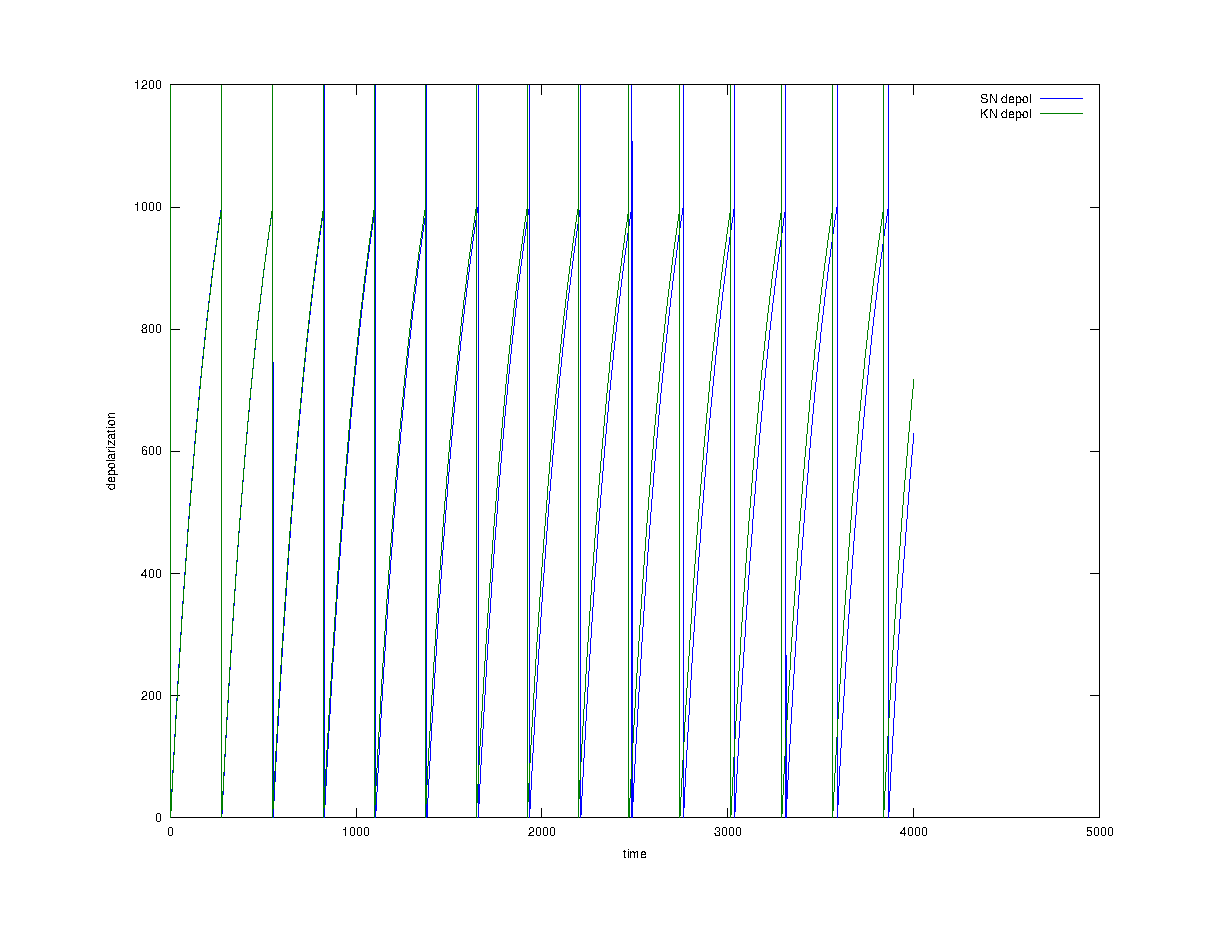
\includegraphics[width=0.95\textwidth]{eps_comparison_between_KN_and_SN_ConstKappa.eps}
	%\end{center}
	\caption{The depolarization curve for a SANN node and a $\kappa$ANN node with the same input. The sensor function has an input equivalent to an activation level of $\kappa = 1.5 \tau$ for both nodes.} %XXX Eller for begge nodeModeller
	\label{figComparisonBetweenSsensorAndKsensorDepolCurveCONStActivityLevel}
\end{figure}

The depolarization of a neuron have a discontinuity when the neuron fires an action potential. 
When the neurons depolarization reaches the firing threshold the value is reset to $v_0 = 0$.
In other words, each time the value of a node reaches a positive threshold, the value is reset.
In this case the global trunctation error will continue to grow, and the difference between the value curves for the SN and the $\kappa$N continues to grow. %TODO Ikkje dette. Skriv heller eit utfall som Stavdahl vil syns er SKUMMELT!

To se if this is the backgound for the error, we isolate the error by giving the sensor aurons a constant sensor function, with an activation level of $\kappa = 1.5 \tau$.

The result is presented in fig. \ref{figComparisonBetweenSsensorAndKsensorDepolCurveCONStActivityLevel}. % .eps
If the previous analysis of the problem is sound, the SN should have a depolarization that is higher than is should be.
This implies than the depolarization curve for the SN would be ``before'' that of the $\kappa$N, which is the opposite of the situation of fig. \ref{figComparisonBetweenSsensorAndKsensorDepolCurveCONStActivityLevel}.





	\subsection{Rounding errors}
%TODO Skriv om: Ikkje røp løysing først. La det være litt spenning!
After a more thorough analysis of the error, it seems that the difference is an effect of a rounding error.

If we change wievpoint on the error and see the difference between the two cuves as an effect of time, we can say that the $\kappa$N's depolarization curve lies before the SN's depolarization curve.
This implies that the $\kappa$N fires before the SN, and thus starts earlier on the depolarization for the next period.

In many programming languages a float is always ``rounded down''. This means that the DECIMAL %XXX FINN RETT ORD: Det som står etter komma TODO
	is removed from the number, and the integer becomes the same as the integer part of the number.

%TODO Viktig: Hugs å skrive om kvifor eg valte en mindre periode i starten av sensor-funk. Dette er viktig, ellers trur han nok at eg bruker dette for å skjule feilen..
\begin{figure}[hb!tp]
	\centering
		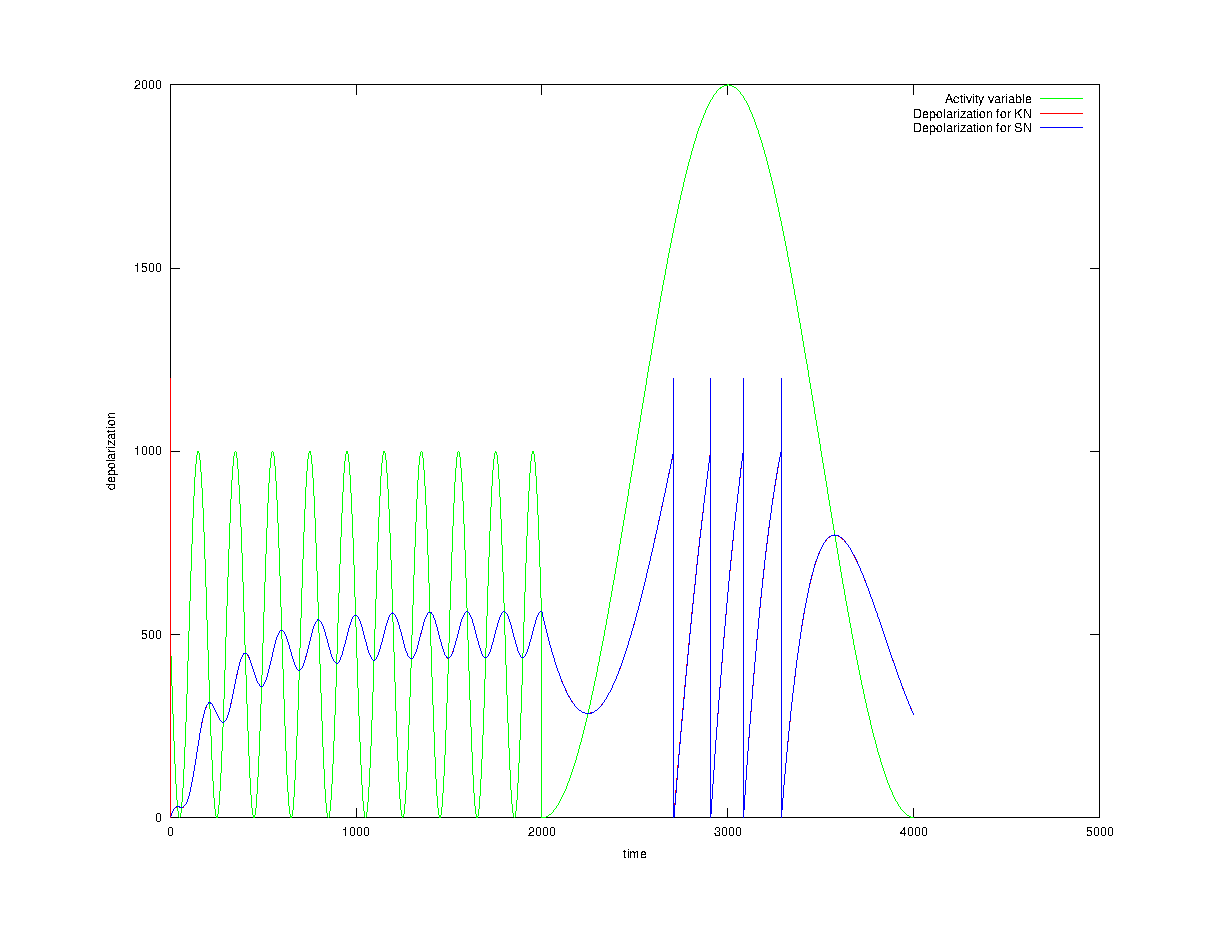
\includegraphics[width=0.95\textwidth]{eps_Comparison_between_the_two_sensors__depol_FIKSA.eps}
	\caption{Comparison between the SN's and $\kappa$N's depolarization curve. The sensor function is plotted in green for analysis purposes.}
	\label{figComparisonBetweenSsensorAndKsensorDepolCurveFIXEdError}
\end{figure}

When the $\kappa$N calculates the estimated firing time, this calculation is done in a double precision floating point number. 
To use this in the scheduler is must first be transformed to an integer variable. When this time step arrives, the task is executed.

%TODO Skriv at vi vil heller runde til nermeste integer, opp om det er best.
% Så skriv korleis dette gjøres, så finn rett kurve.
% TODO analyser frem og tilbake om kor feilen ligger. Det er fortsatt mulig at feilen er for KANN (men trur ikkje det. Legg at feilen er maks når subthreshold polarization er størst. Osv.) XXX
If we instead round to the closest integer, by adding $0.5$ to the float before it is converted into an integer, we get the depolarization curve presented in fig. \ref{figComparisonBetweenSsensorAndKsensorDepolCurveFIXEdError}.
In the improved depolarization curves for the auron, the error is small and can not be seen on the plot.

%Ikkje heilt sikker på om det er heilt rett: størst etter "rising flank of the ..", Bli heilt sikker på dette.
The error is found to be largest right after the rising flank of the activity variable's curve. %TODO ta vekk:   [ , the value of the sensor function. ] ?
For the situation in fig. \ref{figComparisonBetweenSsensorAndKsensorDepolCurveFIXEdError} this is at time t=3000.
At this time iteration the value of the SN is 1.015 more than the value of the $\kappa$N. 

This deviation is substantially smaller that the deviation originating from the rounding error, but it indicates that the analysis made in the previous subsection is correct. %gjør om: ikkje "correct" men kanskje mindre påståelig?
%TODO Skriv analyse av denne feilen, og peik på mulige scenarioer.


% TODO KANSKJE :   \subsection{Floating point calculation pitfalls}
%                  Skriv om mulighetene for feil når man bruker float/double.


% - integralfeil for SN
% - Integralfeilen kommer antagelig av at lekkasjen  
% - For SN vil lekkasjen regnes ut fra verdien ved forrige tissteg. Denne diskretiseringseffekten vil forplante seg i at for positiv derivert av depol-kurva vil SN-depol være litt over, og for negativ flanke : motsatt.
% 		Dette er fordi lekkasjen regnes ut fra forrige verdi, som for stigende flanke er mindre enn den noværande verdien, og vi får en mindre lekkasje => for stor verdi.
% - denne feilen vil nulles ut for eit periodisk signal uten sprang (over en periode vil integralet av positiv flanke og neg. flanke bli null.
% - dersom vi har eit sprang, eller enda verre: eit sprang som alltid ligger etter en viss mengde med pos. flanke, vil vi få summert opp integral-feilen.
% For auronet vil depol settes lik 0 etter en viss mendge pos. flanke for depol. kurva. Dette skaper problemet.

% Eg har også vurdert om det er feil fra implemenasjonen: at de har ulik refraction time, MEN eg trur ikkje dette: 
% 		En slik feil ville vore mindre (eit-to tidssteg per fyring) => ikkje synlig på eit plott over fleire tusen iter's.

% Den lille forskjellen mellom s_sensor_auron og K_sensor_auron er noko eg kan skrive mykje om i 'discussion'.
% Eg har tanker om at det er pga. at eg bruker integer (tid) i ligningene, og vi får dermed avrundingsfeil. Litt overraska over at feilen er så liten..
% 	Det er også mulig at den lille forskjellen kommer av forskellane i korleis sensor-funksjonen blir oversatt til depol.
% 		- K_sensor_auron oversetter sensorFunk direkte til aktivitetsVariabel Kappa, mens
% 		- s_sensor_auron sender gir eit enkelt input per tidsiterasjon gitt av ligninga (W_ij / [time constant]), eller  ALPHA * W_ij
%   XXX Dette trenger grundigare analyser!

% Svaret var: avrundingsfeil av casting fra float til unsigned (fra estimering av tidssteg til Tidssteg). Dette ble alltid runda ned. Løste ved å +0.5 før casting. Funker drita bra!



%TODO Flytt denne tilbake til KANN: det er en aktiv del av implementering. I starten av avsnittet: skriv kvifor eg valte å ha den under design og implementasjon: at det er en aktiv del av utviklinga.
% 		I tillegg finner vi trunctation error: dette blir viktig i diskurs! Kan dermed avslutte å snakke om det i dette kapittelet, og ta det igjen (overraskende) i diskurs--biten:
% 			Det eg tenker på er opdagelsen av at SANN har trunctation error, og at denne vil vakse mot infty.
% 			Diskuter, men end opp med at feilen er liten, og vil ikkje være dødelig..













	\subsection{Analysis of Synaptic Transmission as the derived}
			%\subsection{Analysis of synaptic transmission as the derived}
			\label{ssecAnalysisOfSynTransAsTheDerived}
			To avoid summation of the transmission of all node's input synapses, the edge transmission is defined as the derived.
			To update the synapse's $\kappa_{ij}$, the edge transmission only has to be added to the previous $\kappa_{ij}$. %ta med?  :   that is the change of the synapse's transmission   før "only"?
			As a node's activity variable $\kappa_i$ is defined as the sum of all the input transmissions, $\kappa_{ij}$,
				the postsynaptic activity variable is also updated by summing it with the new edge transmission.

			After each transmission we get the updated $\kappa_i$ as a sum of the current $\kappa_i$ and the edge transmission $u_{ij}(\kappa_j)$
			\begin{equation}
				\kappa_i = \kappa_i + u_{ij}(\kappa_j)
			\end{equation}
			
			After at the end of the time iteration, the effect of the updated $\kappa$ is calculated.
			As the synaptic transmission, and thus the edge tranmission, depend on some of the variables calculated in \emph{K\_auron::doCalculation()}, the updated $\kappa_i$ is first propagated after this function is executed.
			%XXX ? MED? : For an analysis of the time of propagation of $\kappa$ it is referred to section ?. %TODO TODO TODO OTODO OTDO TODO TODO TODOD TODO Skriv in referanse nå er har skrevet om dette i Analyse-kapittelet.

			In fig. \ref{figEdgeTransmissionKaboveT} we can se a plot of the edge transmission of an inhibitory synapse.
			The presynaptic node's activity variable varies as \mbox{$f(t) = 1.1 \cdot \tau \cdot (1 + sin( 2\pi \cdot \frac{t}{1000})$}.
	
\begin{figure}[hb!tp]
	\centering
	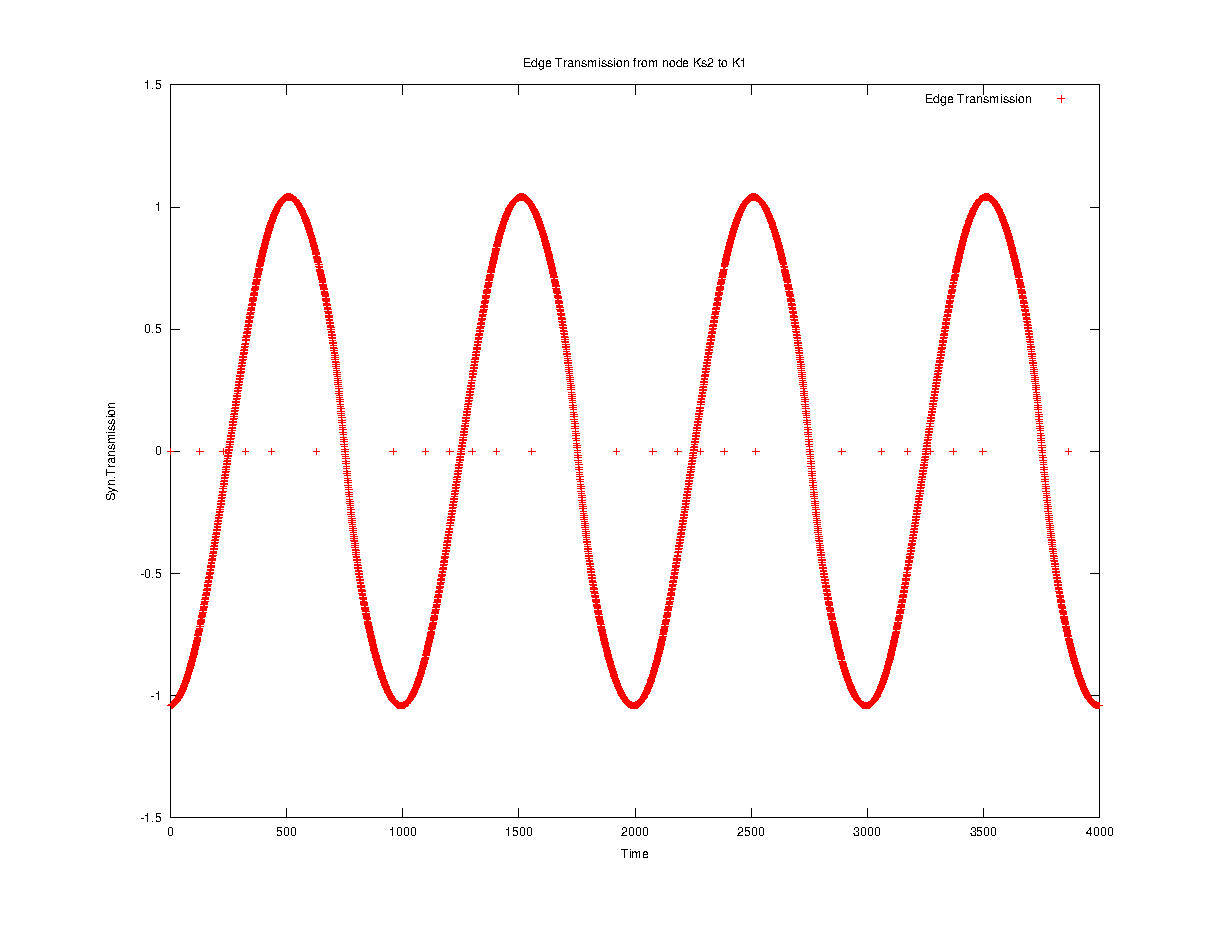
\includegraphics[width=0.95\textwidth]{./synapticTransmissionPlots/eps_transmissionKappaAboveThreshold.eps} 	
	\caption{ 	
			} %TODO skriv om dette tomrommet i teksten under.
	\label{figEdgeTransmissionKaboveT}
\end{figure}

			The edge transmission for an inhibitory synapse is the negative of that of an excitatory synapse.
			From fig. \ref{figEdgeTransmissionKaboveT}, we can therefore see that the synapse is an inhibitory synapse as it shows a plot that resembles $ - 1.1 \cdot cos(x)$, 
				or the negative of the derived of $\kappa_j$.
			%From the figure we can se that the synapse is an inhibitory synapse, as the figure shows a scaled version of the negative of the derived of the presynaptic activity variable.
				%edge transmission is the derived of the presynaptic node's activity variable.

			
			If we let the presynaptic activity variable ``dip'' below threshold, the synaptic transmission becomes zero.
			This is because the period becomes infinitive (the node will never fire) for a sub--threshold activity variable. 
			As the synaptic transission is the synaptic weight times the inverse of the period, the synaptic transission is zero when $\kappa$ is less than $\tau$.
			For the edge transmission we will therefore se see a non--linearity if the activity variable is less than or equal to the threshold.

	% Feil ref.		In fig. \ref{figEdgeTransmissionKaboveT} we can se a plot of the edge transmission of an inhibitory synapse.
	% Feil ref.		The presynaptic node's activity variable is presented in fig. \ref{figEdgeTransmission:edge-a}.

\begin{figure}[hb!tp] 				% TODO TODO TODO TODO TODO TODO TODO TODO TODO TODO TODO TODO TODO TODO FLYTT til resultat og sammenlign. kap.
	\centering
	%
   	\subfloat[Presynaptic activity variable, {$\kappa_j$}]{\label{figEdgeTransmission:edge-a} 						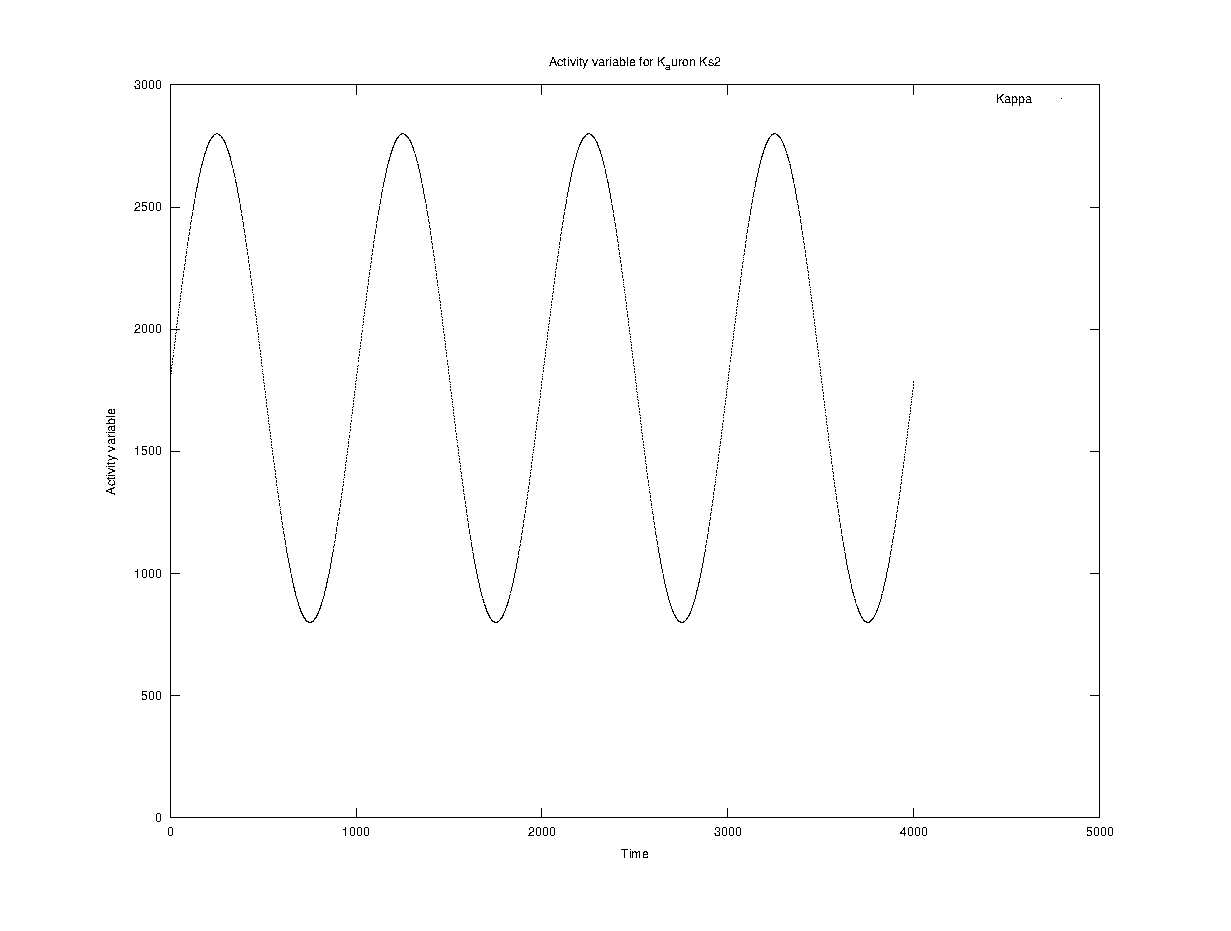
\includegraphics[width=0.95\textwidth]{./synapticTransmissionPlots/eps_auronKs2-kappa.eps} 		}  \\
   	\subfloat[Synaptic transmission]{\label{figEdgeTransmission:edge-b} 		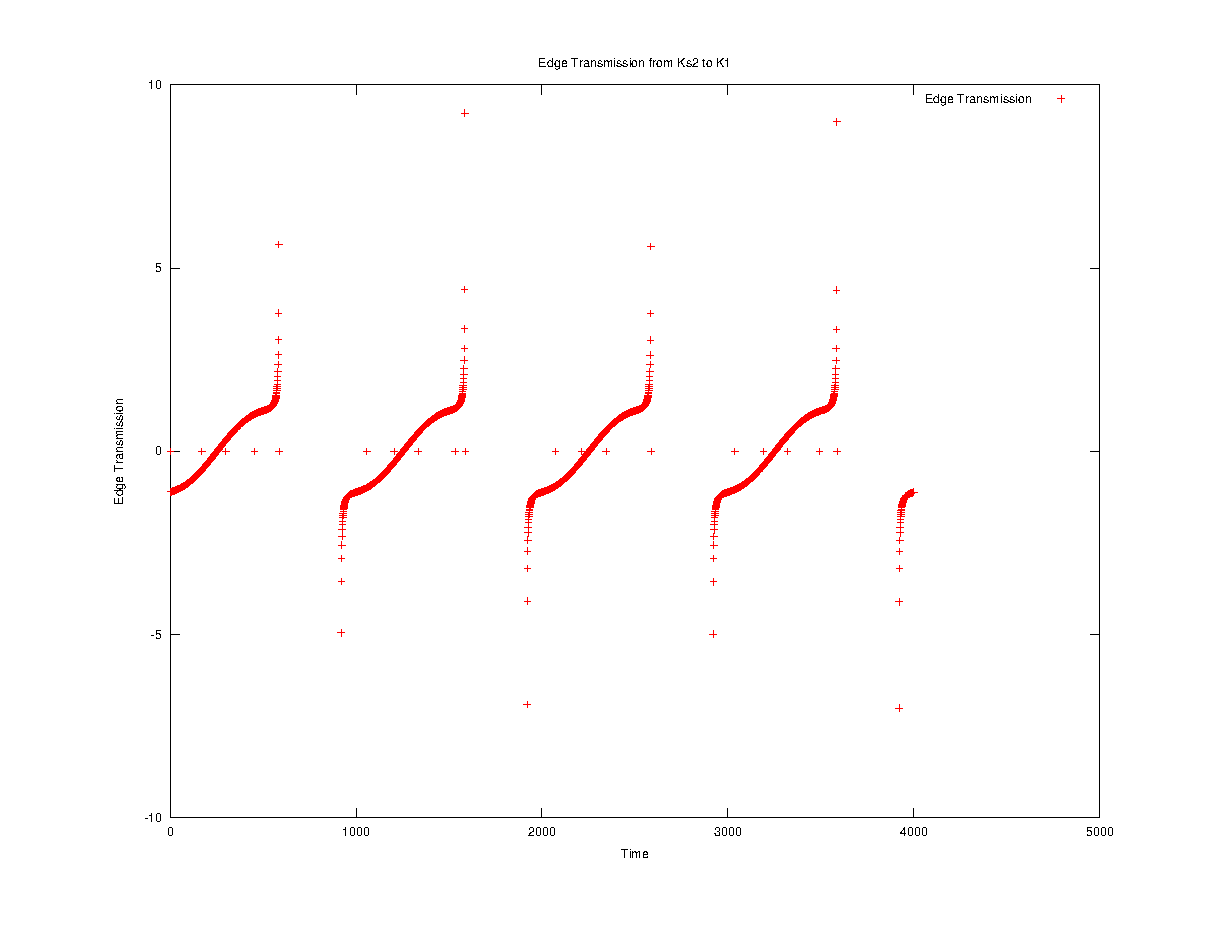
\includegraphics[width=0.95\textwidth]{./synapticTransmissionPlots/eps_transmission_Ks2->K1.eps} 	}
	%\caption{Demonstration of the value function for changing kappa}
	\caption{ 	( \ref{figEdgeTransmission:edge-a} ) The presynaptic activity variable $\kappa_j$         and   
				( \ref{figEdgeTransmission:edge-b} ) The corresponding edge transmission to a presynaptic activity variable presented in \ref{figEdgeTransmission:edge-a}. 
			Notice the gap of the synaptic transmission when $\kappa_j \leq \tau$ = 1000. 
			} %TODO skriv om dette tomrommet i teksten under.
	\label{figEdgeTransmission}
\end{figure}
			If the presynaptic node is a sensor neuron with a sensor function varying as a sinus that dips below threshold, we get the edge transmission presented in fig. \ref{figEdgeTransmission:edge-b}. 
			The presynaptic activity variable is presented in fig. \ref{figEdgeTransmission:edge-a}.

			We can see that the edge transmission no longer resembles the derived of the presynaptic activity function. 
			Now we have a strong non--linearity when $\kappa_j \leq \tau$.
			In all plots in this report, the firing threshold is set to $1000$

			The plots of synaptic transmission is made by running the octave log--scritps resulting from the execution of the implementation.
			In the constructor of each synapse object, a file stream is created. 
			This writes a fully executable octave script. The above plots have been made by executing such scripts.

			%Skriv om at dette er ei inhib. syn. Dette er grunen til at kurva er "opp ned".

	
			% DÅRLIG: Skriv om, men bruk mindre ord, meir følelser, osv. Skal ikkje være veldig teknisk, men skal innlede lese mot neste section.. XXX TPOD COTO DOTO TODO TODO TODO
			By defining the edge transmission as the derived where we integrate all the input in the postsynaptic node involves one drawback, the global truncation error.
			At every step we sum the current value with the new value. If we get a small error in these calculations we get what is called ``truncation error''.






%TODO Flytte analyse over, over til comparison and  results? nee..
%TODO synaptisk transmission overføringsplott, som viser pre og postsyn aktivitetsvar.? Eit som ikkje har problemer: for å vise at det funker..








		% Her skal plottet som gir det mest komplekse responsen ligge (ulineariteten og pausa).
	\subsection{Analysis of the postsynaptic activity variable as a result of syn. transmission} % KANSKJE
	\subsection{etc.}
\section{etc.}

%XXXXXXXXXXXXXXXXXXXXXXXXXXXXXXXXXXXXXXXXXXXXXXXXXXXXXXXXXXXXXXXXXXXXXXXXXXXXXXXXXXXXXXXXX
\section{En hovedforskjell: mulighet for rekalkulering av aktivitetsnivå}
	For simulering fekk vi forskjell i den transiente depol. kurva, mellom de to modellane.
	Mi tolking var at denne feilen er en integralfeil for SN. Feilen økte for større stigning på depol-kurven, og minka til en negativ feil på synkende kurve.
	
	Dersom vi har en kurve som svinger rundt eit arbeidspunkt, så vil feilen for den stigende biten av kurven forsvinne når kurva synker igjen. For en "periode" (dersom det er periodisk, uten sprang) vil feilen integreres opp til å bli 0.

	Dersom vi har eit sprang 
%XXXXXXXXXXXXXXXXXXXXXXXXXXXXXXXXXXXXXXXXXXXXXXXXXXXXXXXXXXXXXXXXXXXXXXXXXXXXXXXXXXXXXXXXX
